\documentclass{beamer}

\newcommand{\norm}[1]{\left\lVert #1 \right\rVert}

\title{An analysis and verification of the efficacy of using Fast Weights with RNNs}
\subtitle{CSE847 (Machine Learning) Project Final Report}
\author{Eric Alan Wayman\inst{1} \and Adi Mathew\inst{1}}
\institute[Universities Here and There] % (optional)
{
  \inst{1}%
  Department of Computer Science and Engineering\\
  Michigan State University
}
\date{April 26, 2017}
\subject{Computer Science}

\begin{document}

\frame{\titlepage}

\begin{frame}
  \frametitle{RNN basics}
  \begin{definition}
    A \emph{standard RNN} is defined by the following equations:
    \begin{align*}
      a(t) & = b + W h(t-1) + U x(t) \\
      h(t) & = \mbox{activ}(a(t)) \\
      o(t) & = c + V h(t) \\
      \widehat{y}(t) & = \mbox{softmax}(o(t))
    \end{align*}
  \end{definition}
  where we choose to minimize the cross-entropy cost function since we are performing a classification task:
  \begin{equation*}
    E = -\ln(p) = -\sum_{\tau=1}^t \sum_{j=1}^k y_{\tau k} \ln\left(\widehat{y_{\tau j}}\right) = \sum_{\tau=1}^{t} E_t
  \end{equation*}
\end{frame}

\begin{frame}
  \frametitle{RNN basics}
  For the associative retrieval task, we wish to only look at the end-of-sequence $y_t$ so the error function becomes
  \begin{equation*}
    E = -\ln(p) = \sum_{j=1}^k y_{t k} \ln\left(\widehat{y_{t j}}\right) = E_t
  \end{equation*}
\end{frame}

\begin{frame}
  \frametitle{RNN basics}
    \begin{align*}
      a(t) & = b + W h(t-1) + U x(t) \\
      h(t) & = \mbox{activ}(a(t)) \\
      o(t) & = c + V h(t) \\
      \widehat{y}(t) & = \mbox{softmax}(o(t))
    \end{align*}
  Note that $W$ and $U$ when chosen with gradient-training procedures will choose $W$ and $U$ that influence $h_t$ such that $E_t$ over the entire batch is minimized (i.e. the ``average error'') is small. Can we do better?
\end{frame}

\begin{frame}
  \frametitle{Associative memory basics}
Consider an associative memory which learns the single key pattern $f$ and value $g$ where both are column vectors (Anderson, \emph{An Introduction to Neural Networks}, 1995). We let the system be the matrix

\begin{equation*}
A = \eta g f^T
\end{equation*}
%
The system performs perfectly:

\begin{equation*}
g^\prime = Af = \eta g f^T f \propto g
\end{equation*}
%
since the $g^\prime$ that is recalled is proportional to the value $g$ associated with the input $f$.
\end{frame}

\begin{frame}
  \frametitle{Associative memory basics}
Now consider a set of key patterns $f_i$ and associated values $g_i$ where all $f_i$ are orthogonal (we write $f_i \rightarrow g_i$ to denote the associations). Letting

\begin{equation*}
A_i = g_i f_i^T, \qquad A = \sum_{i} A_i
\end{equation*}
%
we see that again $A$ performs recall perfectly since for all $j$,

\begin{align*}
  A f_j & = \sum_{i}A_i f_j = \sum_{k \neq j} A_k f_j + A_j f_j \\
  & = \sum_{k \neq j} g_k f_k^T f_j + \eta g_j \propto g_j
\end{align*}
%
\end{frame}

\begin{frame}
  \frametitle{Associative memory basics}
  Using outer products to create memory storage is referred to ``the generalization of Hebb's postulate of learning'' (Haykin, \emph{Neural Networks and Learning Machines} 2009) since weight updates in Hebbian learning are calculated with outer products.

  \vspace{0.5cm}

  Note that generally, not all sets of key patterns would be orthogonal; we discuss the implications of this when we consider the associative memory structure from the Fast Weights paper.
\end{frame}

\begin{frame}
  \frametitle{Dynamic systems approach}
  The RNN is a nonlinear dynamic system defined by difference equations. We focus on the hidden states $h_t$. Since $h_t$ changes not only due to past values of $h_\tau$ but also new inputs coming in at every time step, $x_t$. Thus it is a \emph{nonautonomous} system and stability results for autonomous dynamic systems do not directly apply.

  \vspace{0.5cm}

  However the concepts of \emph{attractors} and \emph{basins of attraction} are useful to understand the behavior of the network. For the most simple type of attractor, the equilibrium point attractor, the \emph{basin of attraction} of an equilibrium state $\overline{x}$ is the set of all $x$ such that $x(t) \to \overline{x}$ when $t \to \infty$ (for our network, the $x$ are $h_\tau$ for $\tau \leq t$.
\end{frame}


\begin{frame}
  \frametitle{Dynamic systems approach}
  When discussing stability for such a network, we are referring to the stability of the hidden unit $h$.

    \vspace{0.5cm}

  We consider

\begin{equation*}
h(t) = \mbox{activ}(a(t)) = \mbox{activ}(b + W h(t-1)) = M h(t-1)
\end{equation*}
%
where $M$ is the map taking $h(t - 1)$ to $h(t)$ for the system where $Ux(t)$ is not included (so the system is autonomous). By defintion for a given $W$ the $h_\tau$ are in the basin of attraction corresponding to the attractor $h_t$ since they approach $h_t$. In practice, if $h(0)$ and $W$ are initialized properly, we may be able to guarantee $h$ will begin in the correct basin of attraction (that of the $h_t$ we want).

\end{frame}

\begin{frame}
  \frametitle{Vanishing gradients in RNNs}
  We summarize the argument of Bengio et al. 1994 which is restated in Hochreiter 2001. They show that even a nonautonomous system like the RNN will converge to the attractor as long as it begins in an area called the reduced attracting set $\gamma$. However, even if the state of the hidden units are in the basin of attraction $\beta$, if they are not in $\gamma$, the state may drift away from the attractor (figures from Haykin 2009).

\begin{center}
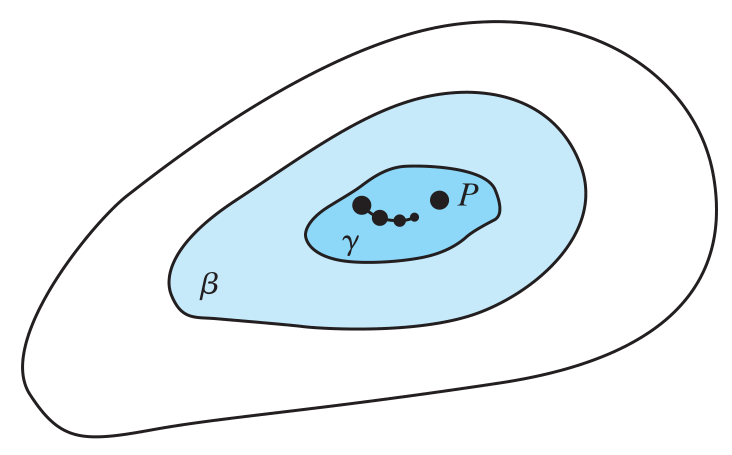
\includegraphics[scale=0.20]{bengio_picture.png} 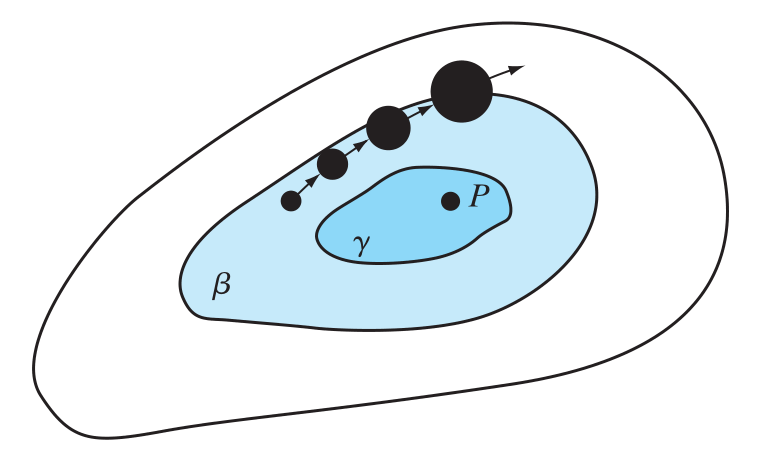
\includegraphics[scale=0.20]{bengio_picture2.png}
\end{center}

\end{frame}

\begin{frame}
  \frametitle{Vanishing gradients in RNNs}
  The authors show that unfortunately, in the region $\gamma$, the gradient of the current state $h(t)$ with respect to $h(\tau), \tau \ll t$ decays quite rapidly. This is an issue because gradient-based training methods, the update to the weight matrix $W$ is adjusted in proportion to these gradients. So, ironically, when the system is in the desired reduced attracting set, we cannot properly train the network, and when the system is not in that set, the weight matrix may change in undesired ways.

\begin{center}
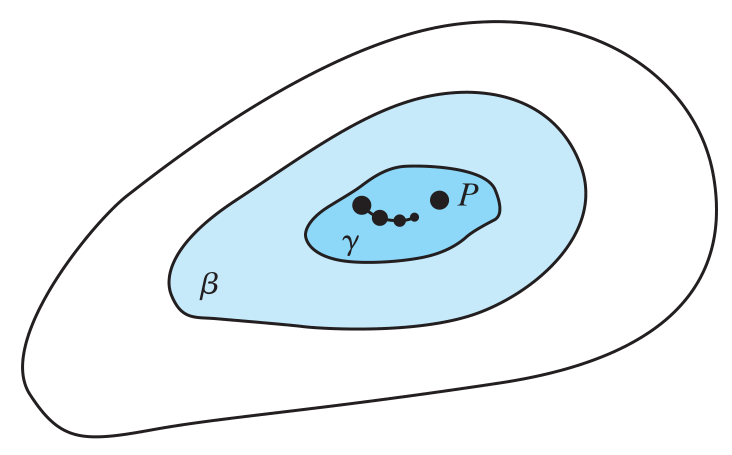
\includegraphics[scale=0.20]{bengio_picture.png} 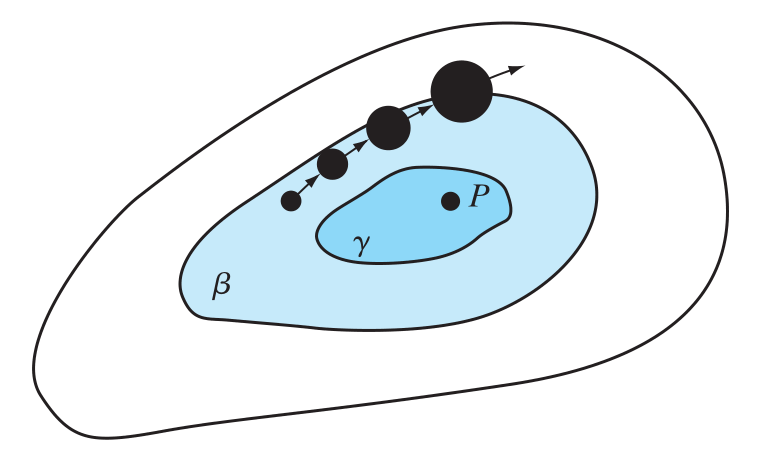
\includegraphics[scale=0.20]{bengio_picture2.png}
\end{center}

\end{frame}

\begin{frame}
  \frametitle{Backpropagation in RNNs}
  \begin{align*}
  J_{W} E_t & = (J_{a_t} E_t)(J_W a_t) \\
  & = (J_{a_t} E_t)(h_t + J_W h_{t-1}) \\
  & = (J_{a_t} E_t)h_t + (J_{a_t} E_t)(J_w h_{t-1})
\end{align*}
%
  The second term cannot be reformulated to include $J_{a_{t-1}} E_t$ since the chain of derivatives has been ``broken'' (i.e. $J_{h_{t-1}} a_t$, the ``connecting term,'' does not appear).

  \vspace{0.5cm}

  A solution to this is to use the notation $W_t$ to represent the $W$ appearing at each time step (Goodfellow et al. 2016, p. 386). Using this notation, $J_{W} E_t$ becomes

  \begin{equation*}
    J_{W} E_t = \sum_{\tau=2}^{t}  (J_{a_\tau} E_t)(J_{W_\tau} a_\tau)
  \end{equation*}

\end{frame}

\begin{frame}
  \frametitle{Backpropagation in RNNs}
\begin{align*}
  J_{a_t} E_t = \delta_{t}^t
\end{align*}

\begin{align*}
  J_{a_{t-1}} E_t & = (J_{a_t} E_t)(J_{h_{t-1}} a_t)(J_{a_{t-1}} h_{t-1}) = \delta_{t}^t (J_{h_{t-1}} a_{t})(J_{a_{t-1}} h_{t-1})  = \delta_{t-1}^t
\end{align*}

\begin{align*}
  J_{a_{t-2}} E_t & = (J_{a_{t-1}} E_t)(J_{h_{t-2}} a_{t-1})(J_{a_{t-2}} h_{t-2}) \\
  & = \delta_{t-1}^t (J_{h_{t-2}} a_{t-1})(J_{a_{t-2}} h_{t-2}) = \delta_{t-2}^t
\end{align*}

So once $\delta_{t-1}^t$ has been calculated, the calculation of the Jacobian with respect to the preceding time step requires the calculating only three Jacobians, rather an ever-expanding product of Jacobians.

\end{frame}

\begin{frame}
  \frametitle{Fast weights augmentation to RNNs}
  The Fast Weights augmented RNN has $h_t$ of the form:
    \begin{equation*}
      h_t^{s+1} = \mbox{activ}\left(LN(b + Wh_{t-1} + Ux_t) + A_t h_{t}^s\right)
    \end{equation*}
    where the superscript $s$ on $h_{t-1}$ is not a power but an index indicating the current iteration of the inner loop ($s \leq S$), and where $LN$ indicates the layer normalization procedure. The $A_t$ term is the fast weights matrix.
\end{frame}

\begin{frame}
  \frametitle{Fast weights augmentation to RNNs}
    $A_t = \lambda A_{t-1} + \eta h_t h_t^T$

    \begin{equation*}
A_{t-1} h_t = \eta \sum_{\tau=1}^{t-1} \lambda^{(t-1) - \tau} h_\tau \left(h_\tau^T h_t\right)
    \end{equation*}

This result is the sum of all past $h_\tau,\, \tau < t$, where each $h_\tau$ is weighted by two quantities:

\begin{itemize}
\item The further in the past is $\tau$, the smaller the magnitude of the resulting vector ($\lambda^{(t-1) - \tau}$ with $\lambda < 1$)
\item The less similar are $h_t$ and $h_\tau$, the smaller the positive magnitude of the resulting vector (the multiple of $h_\tau$ ranges from 1 down to -1, when the vectors are pointed in exactly the opposite direction).
\end{itemize}
%
So $A_{t-1} h_t$ represents the weighted sum of all $h_\tau,\, 1 \leq \tau \leq t-1$ with more recent vectors and vectors more similar to $h_t$ being given higher (more largely positive) weight.
\end{frame}

\begin{frame}
  \frametitle{Fast weights augmentation to RNNs}
  What the above loop does is to influence $h_t$ in a direction towards the vector that results from this sum. Note that without this term, $h_t$ would be influenced by $h_{t-1}$ only through $W$, and influenced by $h_\tau,\, \tau < t-1$ only indirectly through $W$. Thus the effect of the addition of this term causes a $h_t$ to be influenced by all $h_\tau, \tau < t$ directly and in proportion to how recent and how similar each $h_\tau$ is to $h_t$.
\end{frame}

\begin{frame}
  \frametitle{Associative retrieval task}
  \begin{center}
    \begin{tabular}{lc}
      Input string & Target \\
      \hline
      c9k8j3f1??c & 9 \\
      j0a5s5z2??a & 5 \\
    \end{tabular}
  \end{center}
\end{frame}

\begin{frame}
  \frametitle{Associative retrieval task results}

  Results for $R = 50$ for Fast Weights-augmented RNN:
  \begin{center}
  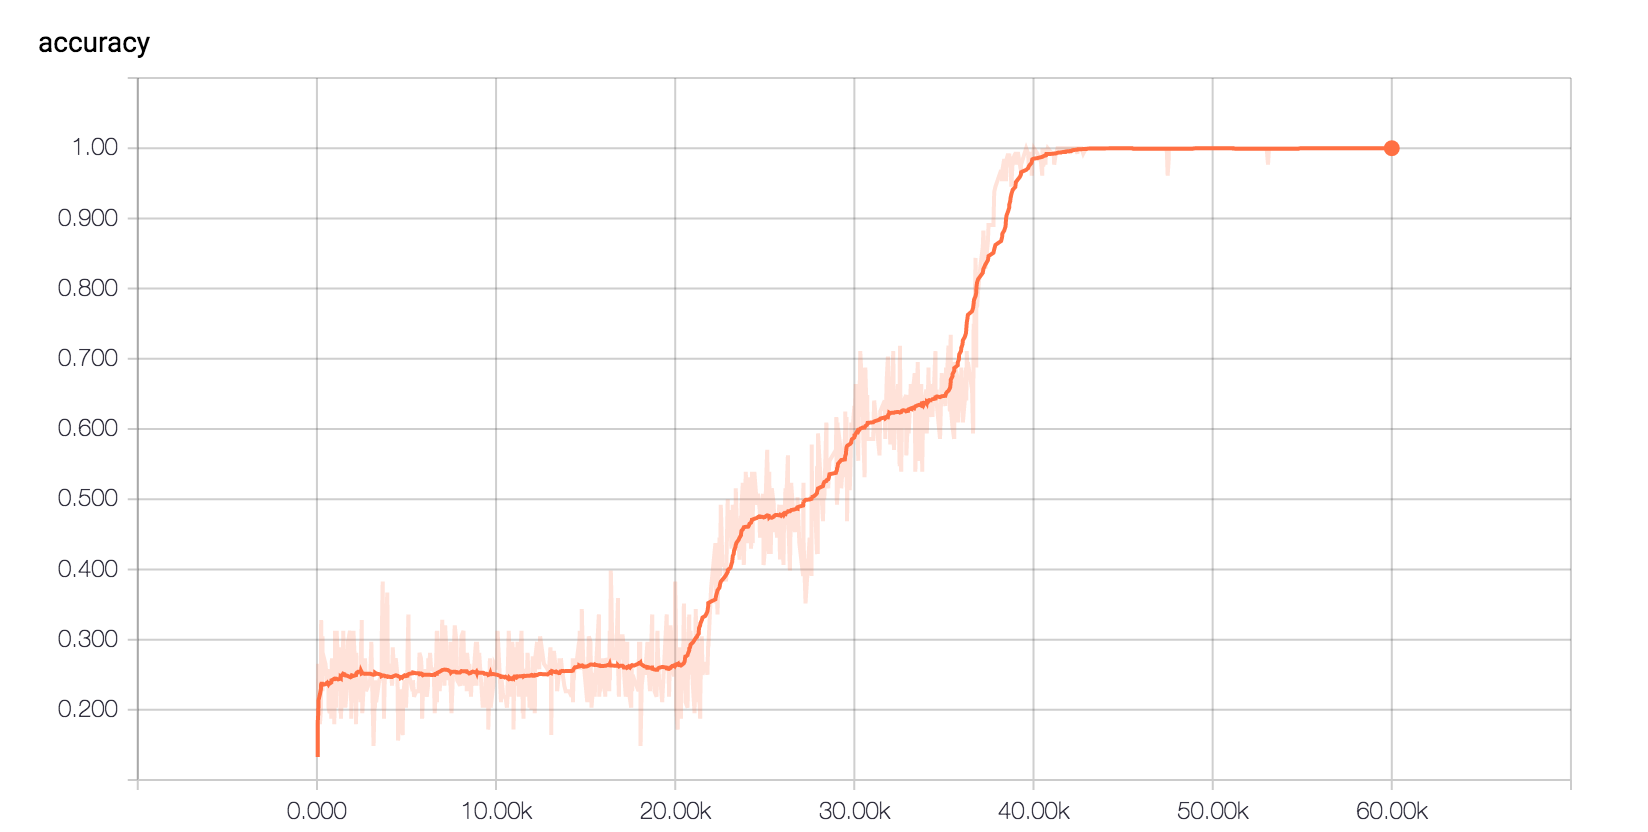
\includegraphics[scale=0.20]{../final/images/fast_weight_r_50_accuracy.png} \\
  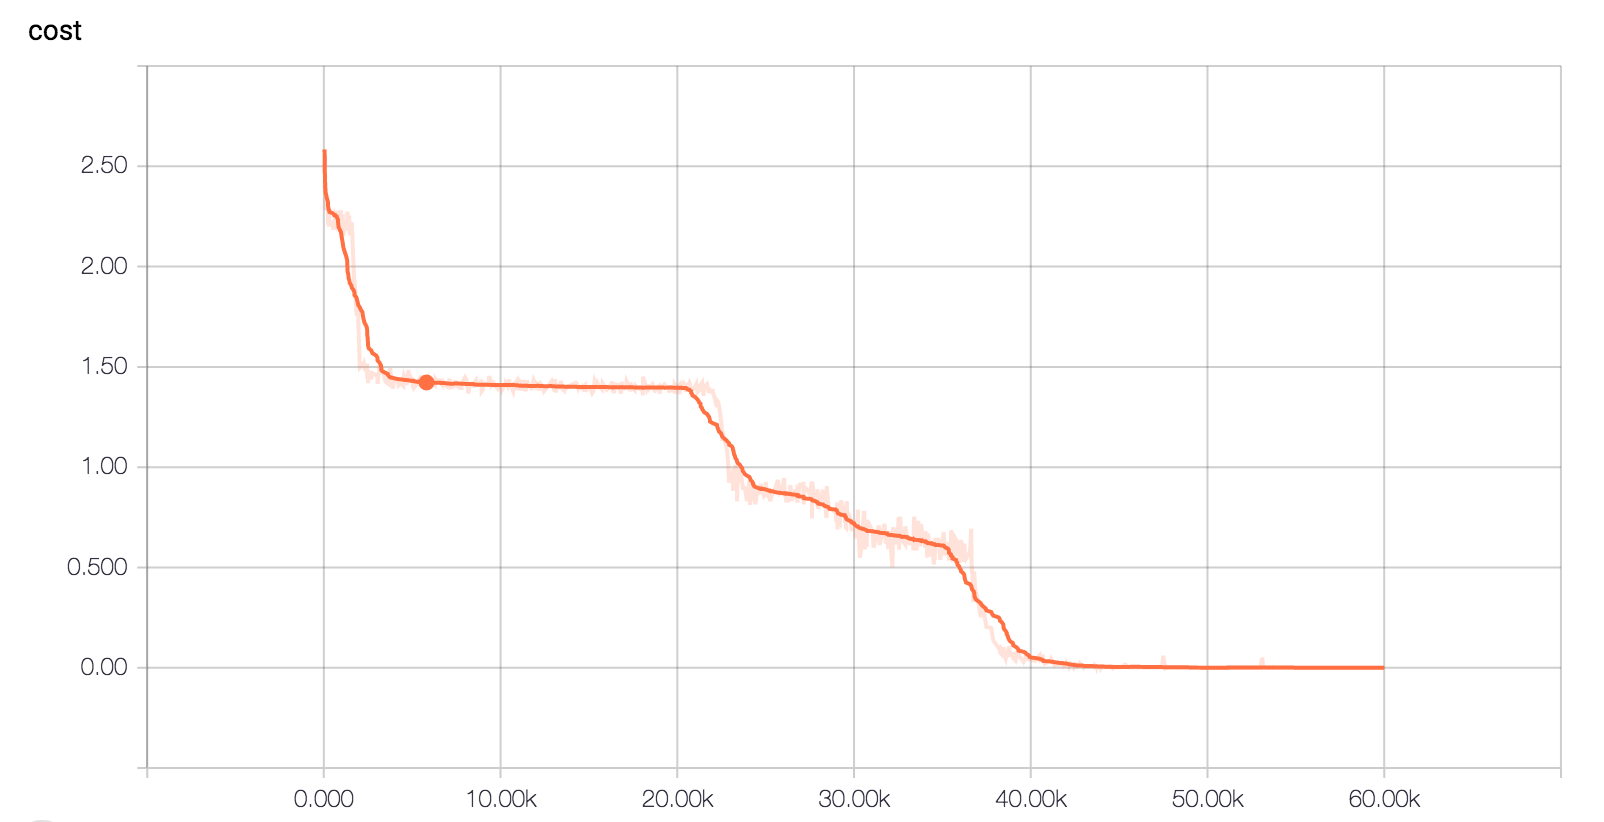
\includegraphics[scale=0.20]{../final/images/fast_weight_r_50_cost.png}
  \end{center}
\end{frame}

\begin{frame}
  \frametitle{Associative retrieval task results}
  \begin{center}
    \begin{tabular}{lccc}
      Model & R = 20 & R = 50 & R = 100 \\
      \hline
      IRNN & 71.2\% & 64.6\% & 3.11\% \\
      LSTM & 53.3\% & 3.88\% & 1.02\% \\
      FW RNN & 3.78\% & 0.00\% & 0.00\%
    \end{tabular}
  \end{center}

\end{frame}

% etc
\end{document}
